\section{Vissim Network Modelling}
\label{modelling}
The Vissim network used throughout the project is derived from a network originally introduced by COWI\footnote{A Danish consulting firm in engineering, environmental science and economics.} and later reworked by DTU Transport students.

COWI's version included ringroad 3 from Jyllingevej to the intersection with highway 3 and even further north. In addition M3, which runs almost parallel with ringroad 3 in this area, was included as well as the minor roads in between..

The network which is modelled in this project is somewhat large. Vissim maintains a \textit{.inp} file, which contains the most relevant informations necessary to run a simulation including information on links, connectors and routes. This file is plain text and can be modified using simple file input-output operations. To properly insert and manage the traffic data necessary to obtain a correct simulation, the inp file is manipulated by scripts - how I do this is explained below\footnote{Note that many of the operations I perform by changing the raw Vissim network data file can be done using the COM interface of Vissim. However when work on this project was commenced only Vissim version 4 was available, which has major flaws in COM interaction. So I decided to take the herein described approach instead, accepting that changes in the Vissim data file format could break my tools. Vissim 5 works much better with COM and future project could involve porting the tools to use the COM interface.}.

\subsection{Modifications and additions to existing model}

As such the network was missing four intersections of O3 from Jyllingevej to Roskildevej. To establish this section satellite photos from Google Earth was combined with intersection layouts, kindly provided by DRD.

The signal plans and naming conventions for the existing intersections in the COWI model for O3 intersections were adopted when entering the four missing intersections into the network. As for the intersection layout, DRD provided the missing signal plans for these intersections as well.

To prevent side-effects all links not connected to O3 from Herlev Sygehus to Jylligevej were removed as well as all parking lots (DTA zones).

A number of mistakes were corrected in the definition of the intersections. This was done using layout plans for the intersections from DRD. Most mistakes were related to non-existent turning-lanes (and even turning possibilities) and the placement of bus-only lanes. 

\subsection{Link inputs}
The original network generated traffic load and route choices from OD matrices. For my simulations I had decided to use static inputs and routes from the traffic counts and detector data, analysed in section \ref{data}. 

Link inputs are created on the basis of the detector data from TTS and the traffic counts from DRD. First the traffic counts is used to establish the proportion of cars to trucks for all approaches, except Ejby Torvevej. Then, for the approaches, which were measured upon in the TTS data, I apply detector values rather than traffic count values. This is done using detectors north of Herlev Sygehus in Herlev and from south for the east-, west- and southern approaches to Roskildevej.

The link inputs were scaled to represent hourly traffic input, as Vissim require, and inserted into the Vissim network file.

The format of a link input in the Vissim inp file is:
\begin{verbatim}
INPUT <input_number>
      NAME "<input_description>" LABEL  0.00 0.00
      LINK <link_number> Q <link_contrib> COMPOSITION <comp>
      TIME FROM <t_begin> UNTIL <t_end>
\end{verbatim}

(Vehicles always arrive at the beginning of the link.)

Where the most important fields are the \textit{link\_number}, defining on which link the input occurs, the \textit{link\_contrib}, which is the input quantity in vehicles per hour and finally \textit{t\_begin} and \textit{t\_end} ie. the time period in which this traffic quantity must be generated.

The \textit{comp} variable defines the traffic composition used eg. cars, trucks, buses or a combination. According to the Vissim manual it is possible, but not recommended, to define multiple inputs on the same link for the same period of time. Since the traffic composition will remain fairly static it is more intuitive to define a single link input for a traffic composition, which defines relative proportions of each possible vehicle type.

\subsection{Routes}
\label{routefractions}
Routes can be designed using the GUI tool provided with Vissim. However, in the spirit of the solution for automated link inputs routes are inserted automatically. 

At every intersection it is possible to follow each adjacent link (ie. turn left, right or go straight through) and thus the total number of routes from an input link to an exit link in the network is tremendous.

To apply traffic count dataset by DRD in Vissim (section \ref{traffic_count_analysis}) it is possible to use Vissim \textit{turning decisions} but the Vissim manual is clear that static routes should be used instead, when modelling turning distributions. The main reason is that congestion may cause a decision to turn to be overruled whereas a vehicle on a fixed route will wait for the congestion to clear. It appears that technical limitations in Vissim (or perhaps backwards compatability requirements) render Vissim unable to fixate a certain destination upon a vehicle by using turning decisions alone, unlike when using a routing decision. But routing decisions has an edge over turning decisions in that they can be made a long time before the vehicle arrives at the critical point at which to turn, allowing the vehicle to position itself in the turning lane rather than making a last-minute lane change, when the turning decision is applied.

The simplest approach was to introduce a routing decision for each approach, which had traffic count data, and then add routes - respecting the counting data - which represented the turning motion. Such a route is \textit{internal} as it does not necessarily lead from an input to an exit link. Consequently this approach yields a network with the possibility of endless circulation of vehicles, however since we only regard an arterial in this project - and the fact that there are no U-turns in the network - no vehicles will be able to circulate and will always find an exit link.

The routing decision must be placed at a \textit{decision point}, however this does not exist in Vissim. Rather the decision point is scattered over 2 or more connectors attached to each link facing an intersection. In order to overcome this these connectors were grouped by a naming convention which identifies which decision point they belong to and which turning motion they will cause a vehicle to take. 
The names are the concatenation of the direction from which traffic arrives (ie. north, south, east or west), the number of the intersection the decision belongs to (intersections are numbered increasingly from north to south) and finally the turning motion (ie. left, through or right), whichever is applicable. 

As an example the decision point at Herlev Sygehus (the northern-most intersection with the number 1), which faces traffic from north consist of three connectors, are called \verb|N1L|, \verb|N1T| and \verb|N1R|.

To find the insertion point for the routing a backtracking search is made from each turning motion until a common link is found. This link is thus the decision point and we can automatically generate our internal routes by using the discovery routine of section \ref{routingdecisions} to find a valid route.

In Figure \ref{fig:flow_dist_principle} is an example of decision points (y) and the proportions of traffic for each turning motion.
\begin{figure}[htbp]
\centering
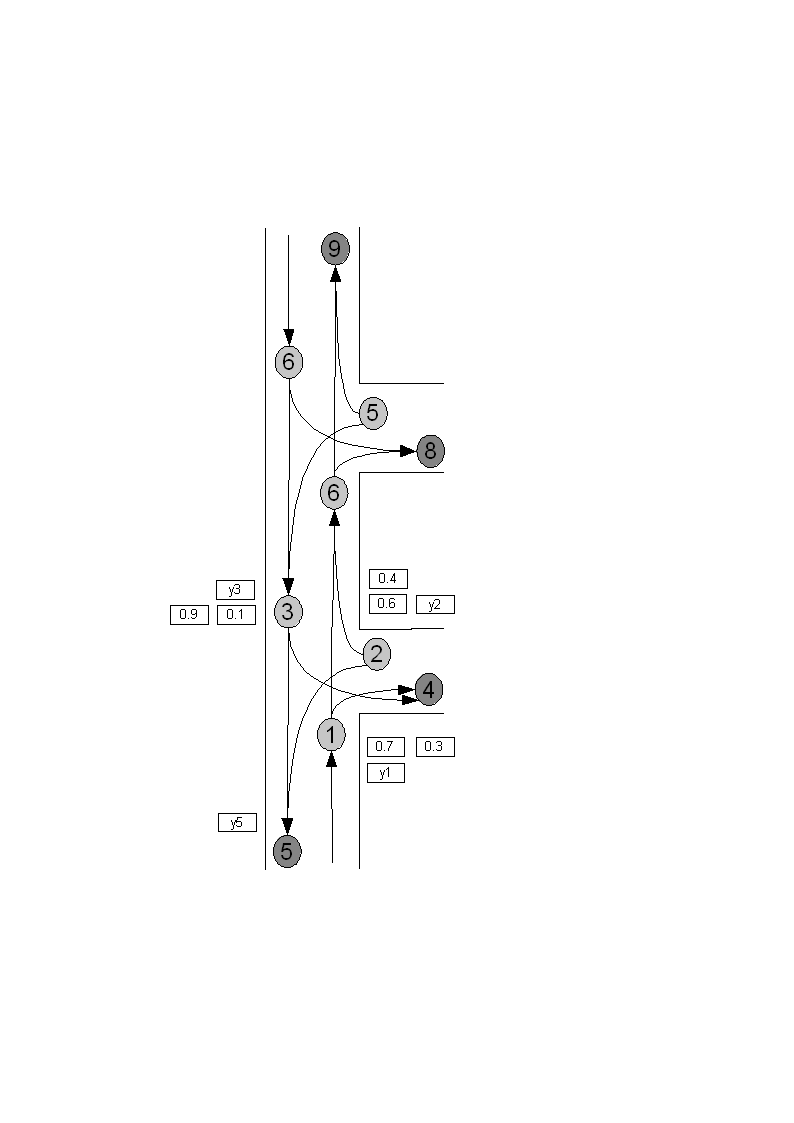
\includegraphics[scale=0.6]{trafficcount_to_routes_sketch.png} 
\caption{Flow distribution principle}
\label{fig:flow_dist_principle}
\end{figure}

In the Vissim network file a routing decisions and the corresponding choice set has the format:

\begin{verbatim}
ROUTING_DECISION <number> NAME "<description>" LABEL  0.00 0.00
     LINK <origin_link> AT 50.000
     TIME FROM 0.0 UNTIL 99999.0
     NODE 0
      VEHICLE_CLASSES <composition>
     ROUTE     1  DESTINATION LINK <dest_link1>  AT   5.000
     FRACTION <fraction1>
     OVER <connector> <link> ... <connector>
     ROUTE     2  DESTINATION LINK <dest_link2>  AT   5.000
     FRACTION <fraction2>
     OVER <connector> <link> ... <connector>
\end{verbatim}

The \textit{origin\_link} denotes the position of the decision point. The line \textit{VEHICLE\_CLASS...} impose a limit of the vehicles, which are required to select on of the routes of this routing decision. A composition may be a single vehicle type (eg. Car) or a combination (eg. Car, Truck). Next comes a number of lines with route alternatives. The \textit{OVER...} lines describe the path taken from \textit{origin\_link} to \textit{dest\_link}. The first connector must be downstream of - and connected to - the decision point link. Likewise the final connector must be upstream and connected to the destination and the same applies to internal links.

The fractions define the relative distribution of vehicles of the given class or classes, which should take each route. Route fractions are taken directly as the values of each turning motion of the DRD supplied traffic counts.

In order to enumerate the relevant routes defining a turning motion it is necessary to parse the \textit{.inp} file and generate an internal representation of the network as a graph. A route discovery routine was implemented:

\begin{verbatim}
def discover start, exits, path = [], &route_found
  return if path.include?(start) # avoid loops
  # check if start is the road segment we search for
  route_found[Route.new(path + [start])] if exits.include?(start)
  if start.is_a?(Connector)
    # you can only search on by going to the connected link
    discover(start.to_link, exits, path + [start], &route_found)
  else
    # start is a link and has zero or more outgoing connectors 
    start.outgoing_connectors.each do |conn|
      discover(conn, exits, path + [start], &route_found)
    end
  end
end
\end{verbatim}

The discovery routine uses recursion to explore the network and find exit links, which are connected to \verb|link| by a path of links and connectors.

In the initial call only the starting link is given along with an empty path and a callback-method, \verb|route_found|, which is invoked by each call timed a new route is found. 

(The \verb|discover| routine is a so-called generator of Ruby and the first invocation might look like this: \verb+discover(start_link){|route| routes.add(route)}+ where the block is enclosed by \{\} and all routes found from \verb|start_link| are simply stored for later in an array.)

A Vissim route is a sequence of connectors and links and must start and end with the first connector, which is outgoing from the start link, and the connector, which is incoming to the exit link, resp.

In line 2 a check is made if the adjacent link, which is currently being explored, has already been visited in which case it should be skipped to avoid a loop. In line 8 it is checked wether the adjacent link leads out of the network. If it does we have found a route from the start link otherwise we descend into the recursion and explore the adjacent links of this link.

The \verb|Route.new| invocation, which is performed when an exit link is found, instantiates a new Route object, which enables additional options such as printing the mentioned sequence of connectors links for Vissim, which is more cumbersome with just the raw path.

\clearpage

\subsection{Right-of-way}
The purpose of a traffic signal is to fairly distribute the right-of-way for conflicting traffic motions.  In spite of this traffic signals cannot overcome all situations and rely on road users to enforce themselves some right-of-way rules. This especially becomes relevant when the capacity of the intersection is reached and vehicles become trapped due to a stage change.

Vissim per default allows "collisions" since overlapping links and connectors must be manually prioritized or marked as a conflict area. The existing network was built using previous versions of Vissim, which only supported priority rules (see Figure \ref{fig:priority_rules}). 

\begin{figure}[htbp]
\centering
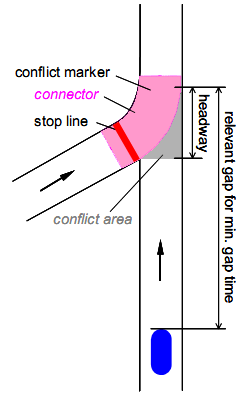
\includegraphics[scale=0.5]{priority_rules.png} 
\caption{From the Vissim manual: illustration of priority rule concepts}
\label{fig:priority_rules}
\end{figure}

In Vissim 5, which was used in this project, there is also the concept of conflict areas, which is recommended over priority rules (the latter remain in Vissim for compatibility) since they are easier to establish and will result in more intelligent driving behaviour. For instance vehicles will avoid entering a conflict area if they can see that it will not be possible to leave it with a certain minimum speed, which will prevent vehicles from clogging up intersections.

Conflict areas and priority rules both rely on threshold values (gap) which road users will use to assess wether it is possible to safely enter a conflict area. The gap is an estimate of the minimum time before the next vehicle from a conflicting link will enter the conflict area.

For the extensions made from Jyllingevej to Roskildevej relevant conflict areas was added for each of the four intersections. The default values in Vissim service pack 6 was used for all conflict areas.

During simulation it became apparent that the priority rules did not prevent collisions in the preexisting intersection so it was decided to replace them with conflict areas. The intersection which had collisions using only priority rules are:

\begin{itemize}
\item Herlev Syghus
\item Hjortespringvej
\item Herlev Hovedgade
\item Mileparken
\item Ejby Industrivej
\item Ejby Torvevej
\item Jyllingevej
\end{itemize}

The intersections with the most observed collisions were Herlev Hovedgade, Hjortespringvej and Herlev Sygehus. It appears that priority rules have difficulties in coping with trapped traffic whereas conflict areas avoid all collisions.
Thus the only priority rules which are carried over from the original model are those for bus stops. 

Conflict areas basically make vehicles in conflicting traffic flows aware of each other so that collisions can be avoided. It is also possible - but not mandatory - to assign a priority. Conflict areas for merging situations should preserve the order of the vehicles and thus have no priority. 

A number of additional situations arise for which the following rules were used:

\begin{enumerate}
\item Left-turning traffic must wait when traffic from the opposite direction - and in the same stage - is going through the intersection
\item When vehicles are trapped in the intersection, waiting for a left turn while the stage changes the vehicles from the next stage, which are in a conflicting motion, must wait for the left-turners to clear even though they have a green light. This is to avoid having traffic stuck in the intersection waiting for their next stage
\item Buses leaving bus stops are always prioritized
\end{enumerate}

\subsection{Signal plans}
Signal plans define the stage sequence, green duration and how changes between adjacent stages should happen with respect to colors in the from and to stages. For cycle-based signal plans the cycle time must be equal to the sum of green and interstage time from the beginning of the first stage until it begins again.

A single stage defines the signal head colors of one or more signal group, which, in turn, is a group of signal heads operating synchronously.

The simplest signal controller consist of two stages. In  Figure \ref{fig:simple_intersection} the arrows indicate the directions being served green.

\begin{figure}[!ht]
\centering
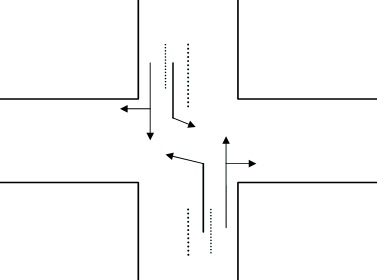
\includegraphics[scale=0.5]{simple_intersection.png} 
\caption{A simple intersection}
\label{fig:simple_intersection}
\end{figure}

DOGS rely on existing signal plans and modify the duration of the stage or stages, which serve green in the direction of the arterial. Thus DOGS assume that the stage sequence and interstages are \textit{optimized} so that the time lost in stage changes is minimized and \textit{safe} so that vehicles in eg. left-turning movements have time to leave the intersection before the conflicting direction receives green.

For this project DRD has supplied a number of signal plans for each intersection, developed by TTS. Throughout the plans signal groups in one direction (usually the major one) are named A and B in the perpendicular direction. Names such as At, Av, Atv indicates signal group for the throughgoing, leftgoing (v = venstre (danish) = left) and a combination for the final name variant. Lower case a's and b's indicate a signal group for pedestrians in the major and minor direction resp. Lower case v's mean that for the controller(s) in this plan a left-turning light is attached to an ordinary red-yellow-green light in order to make it clear that left-turners now have the lane to themselves. If the V is in upper case the light is exclusively for left-turning traffic.

For some intersections a number of alternative plans were supplied. Considering the scope of this project only a single plan was chosen for each intersection and time of day. Generally plans involving pedestrian or bicyclist actuated stages were avoided so as to reduce the complexity of the simulation and maximize the potential for traffic signal optimization. Pedestrians can have devastating effects on vehicular traffic performance on issues of throughput and coordination eg. when a button is pressed to activate a pedestrian signal stage or pedestrians linger too long in a crosswalk. It was confirmed by TTS that pedestrian-actuated stages, which are taken in a stochastic manner ie. when a button is pressed, can be devastating to the coordination of traffic signals. Furthermore multiple through-going bicyclists may hinder the flow of right-turning vehicles (in right-side driven traffic networks) and the handling of these issues are not in the scope of this project.

As a final simplifying step it was chosen not to provide signal heads for pedestrians and bicyclists as these types of road users are not being simulated. Pedestrian stages will mostly follow the parallel stages anyway and if this is not the case then the stage, which is being denied in favor of the pedestrian stage, will simply receive red for the duration.

The final plans, which are used in the simulation, can be seen in appendix \ref{app:signalplans}.

The actual implementation was done in VAP by running the interstages at the cycle second according to the signal plan, for more details refer to section \ref{vap}.

\subsection{Signal controllers}
\label{signal_details}
The optimization system (see Section \ref{eval_coord}) needs some additional information on the signal controllers, the distances between intersections and which stages are arterial. This is not immediately available in the Vissim network file but can be deduced.

Since Vissim does not offer the concept of an intersection - and this is needed to place intersections relative to each other for signal coordination - this information was extracted as follows.

Arterials have the property that they have two major traffic streams, which traverse the arterial from end to end. These streams can be called \textit{up and down} or \textit{left and right} or even \textit{clockwise and counterclockwise}. The point is that there are always two. In this project the streams were called North and South indicating the direction from which they come. We can now find these streams by finding the routes that traverse all decisions (see section \ref{routefractions}), which are through-going and in one of the arterial directions.

For the arterial route from north, we look for a route which reaches the Herlev Sygehus intersection from north and takes the throughgoing turning option \verb|N1T|, the route must then pass through Hjortespringvej \verb|N2T| and so forth until it takes the final decision at Roskildevej \verb|N12T| and exit the network.

\subsubsection*{Distances between intersections}
One of the things we really need to assess the quality of coordinations is the distances between the signal heads (stop-line) for adjacent intersections. The Vissim network file contains information on which link or connector (denoted in common as road segment) each head is placed. By marking all road segments, which are part of the arterial routes, we can deduce which signal heads give green light vehicles travelling in the arterial direction.

The distance from signal controller 1 to 2 is then calculated by summing the lengths of road segments from the arterial signal heads at controller 1 to the arterial heads at controller 2 and so forth.

\subsubsection*{Arterial stages}
This is also a good time to mention the notion of arterial stages. In optimization of coordinations we need to know if a stage is meant for the arterial or for a minor road. And if it is for the arterial, from which direction.

When we calculated distances between intersections on the arterial we learned which signal heads provided for the artery. Since each head is a part of a signal group and a stage is a selection of groups, which are run simultaneously, we can deduce the arterial stages using these rules:

\begin{enumerate}
\item A stage is arterial ie. gives green light to the artery, if it contains an \textit{arterial group}
\item A group is arterial if it contains an arterial signal head
\item And finally, as outlined previously, a signal head is arterial if is placed as on a link, which is marked as arterial
\end{enumerate}

The reason I only require stages and groups to \textit{contain} an arterial group and head resp. is that a stage could contain purely arterial groups and then, maybe, a group for left-turners but the stage is still arterial.

During group naming, when intersections are built, the designers usually prefix the name of the main direction \verb|A| and the side roads \verb|B|. By extracting the definitions of arterial groups as explained above we can see that not all road engineers had the same opinion:

\begin{table}[!ht]
\centering
\begin{tabular}{l|l|l}
 & \textbf{Intersection} & \textbf{Arterial Groups}\\ \hline
1 & Herlev Sygehus & A1, A2\\
2 & Hjortespringvej & A, At\\
3 & Herlev Bygade & A, At\\
4 & Herlev Hovedgade & B, Bt\\
5 & Mileparken & A, At\\
9 & Fabriksparken & A1, A2\\
10 & Gammel Landevej & A1, A2\\
11 & Kindebjergvej & A1, A2\\
12 & Roskildevej & B, Bt\\
\end{tabular}
\caption{Groups for main traffic direction as perceived by traffic signal designer}
\label{tab:arterial_groups}
\end{table}

As can be seen in Table \ref{tab:arterial_groups} the perceived main directions for Herlev Hovedgade and Roskildevej is to-and-fro the city of Copenhagen and western Sealand.

These descriptions conclude on the main issues I have solved in automatic data insertion, manipulation and extraction for Vissim.